\documentclass[10pt,conference]{IEEEtran}
\usepackage{graphicx}
\usepackage{booktabs}
\usepackage{array}
\usepackage{xcolor}
\usepackage{amsmath}
\usepackage{siunitx}
\usepackage[hidelinks]{hyperref}
\pdfpagewidth=8.5in
\pdfpageheight=11in
\title{XORFLOW: Supplementary Evaluation Appendix}
\author{Anonymous Authors}
\renewcommand{\thefigure}{S\arabic{figure}}
\renewcommand{\thetable}{S\arabic{table}}
\newcommand{\sys}{\textsc{XORFLOW}}
\newcommand{\beicsr}{\textsc{BEICSR}}
\newcommand{\DeltaFmt}{\textsc{Delta}}
\newcommand{\xor}{\mathbin{\oplus}}
\begin{document}
\maketitle

\section{Supplementary evaluation scope}
This supplement reports support writes, anchor-lifecycle accounting, structural controls, codec bytes, shared-memory/SCALE-Sim scheduling, held-out Ramulator2 validation, RTL throughput, and physical-design measurements. Producer and consumer anchor sources are accounted for explicitly, every producer recovery precedes target encoding, and one common scheduler is applied to every compatible checkpoint.

\section{Inter-layer structure}
\begin{figure*}[t]
\centering
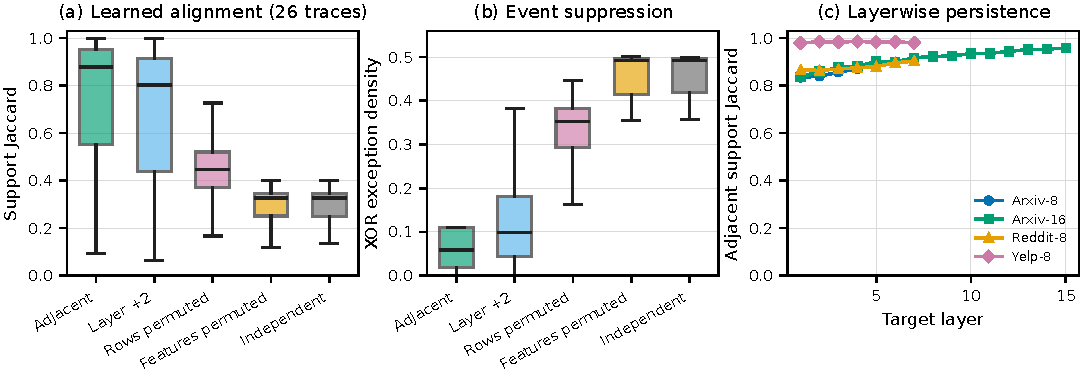
\includegraphics[width=\textwidth]{supplement/figures/figS1_structure.pdf}
\caption{Complete support-persistence characterization. (a--b) Distributions across 26 traced configurations. Real adjacent supports have median Jaccard 0.879 and median XOR exception density 0.0588; exact-count independent controls reach 0.327 and 0.4925. Row and feature permutations destroy most of the advantage while preserving important marginal statistics. (c) Representative layerwise traces show that persistence remains high through residual depth. Source: \texttt{A1\_layerwise\_persistence.csv} and \texttt{A2\_learned\_structure\_controls.csv}.}
\label{fig:s-structure}
\end{figure*}

Figure~\ref{fig:s-structure} directly tests the paper's empirical premise. Exact-count independent masks preserve each layer's number of active positions, yet raise the median event density by $8.38\times$ relative to real adjacent pairs. Row permutation produces median Jaccard 0.447 and forces fallback for essentially every record. Nonadjacent layer $\ell+2$ remains more correlated than random but is consistently weaker than the adjacent pair. The comparison isolates learned positional correspondence from density and within-layer row regularity.

\section{Codec decomposition}
\begin{figure*}[t]
\centering
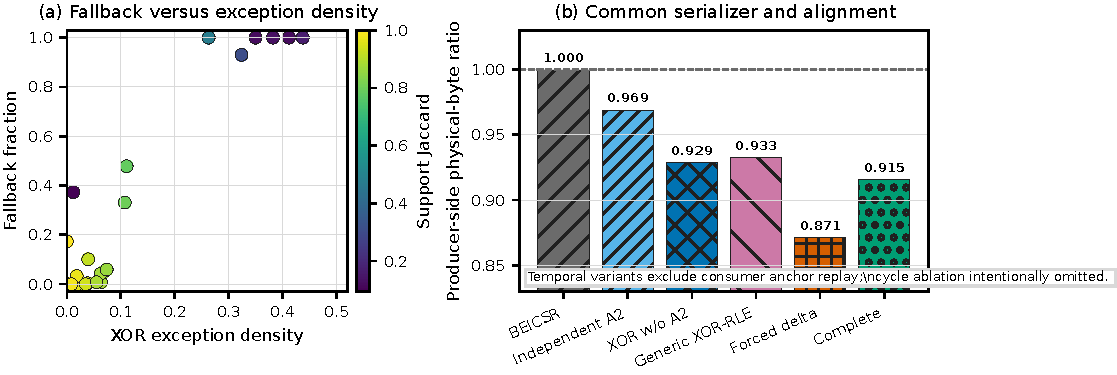
\includegraphics[width=\textwidth]{supplement/figures/figS2_fallback_ablation.pdf}
\caption{Common-accounting codec decomposition. (a) Physical-byte reduction uses the same serializer, padding, unchanged traffic, and consumer anchor bytes for every variant. (b) All variants use common byte accounting; timing comparisons are reported for the baseline and complete \sys{} design. Source: \texttt{results/ablation\_bytes\_only.csv}.}
\label{fig:s-ablation}
\end{figure*}

Independent majority-prototype coding reduces physical bytes by 5.4\% relative to optimized \beicsr{}. Fixed-anchor XOR reaches 10.5\%, generic XOR--gap coding 10.4\%, forced delta 19.6\%, and complete online selection 12.7\%. Temporal coding is therefore the largest increment beyond independent spatial coding. Forced delta is smaller in aggregate but loses local protection and the fixed-partition pair-write bound. The complete \sys{} rows use the same serializer, anchor accounting, and execution model as the primary evaluation. Ablation conclusions are restricted to serialized and physical bytes.

\section{Consumer accounting and dependency audit}
\begin{figure*}[t]
\centering
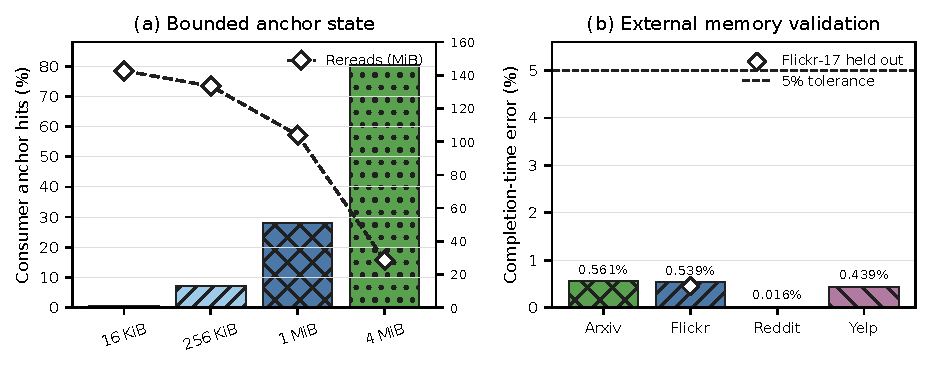
\includegraphics[width=\textwidth]{figures/fig8_final_validation.pdf}
\caption{Lifecycle and external-memory validation. (a) Consumer hit rate rises with anchor capacity while exact compressed rereads fall. (b) Complete retained-stream predictions for Arxiv, Flickr, Reddit, and Yelp remain within 0.57\% of Ramulator2; the Flickr--17 diamond is an independent held-out absolute check. Source: \texttt{results/anchor\_lifecycle\_summary.csv} and \texttt{results/complete\_external\_memory\_validation.csv}.}
\label{fig:s-schedule}
\end{figure*}

The 16-KiB consumer store retains 422 of 72,604 delta anchors (0.581\%); 72,182 recoveries reread 142.67~MiB and consume 1.320 million decode cycles. The producer path independently rereads the same total, giving 285.34~MiB and 2.641 million decode cycles across both lifecycles. At 256~KiB, 1~MiB, and 4~MiB, consumer hits rise to 7.10\%, 27.94\%, and 80.43\%, while rereads fall to 133.46, 103.92, and 28.61~MiB.

The per-record audit reports zero producer-readiness violations across 73,652 targets and classifies every one of the 72,604 delta targets. The common scheduler covers all ten eligible checkpoints plus a 16-layer Arxiv extension and Chameleon control. Its independent max-plus recurrence agrees exactly with every baseline and proposal schedule.

\begin{table*}[t]
\centering
\caption{Final results for every compatible eight-layer checkpoint. Support and physical traffic are exact; cycles are modeled aggregation--combination-subsystem completion times from the common shared-memory/SCALE-Sim schedule.}
\label{tab:s-checkpoints}
\scriptsize
\setlength{\tabcolsep}{4pt}
\begin{tabular}{lrrrrr}
\toprule
Trace & Support reduction & Physical reduction & BEICSR cycles & XORFLOW cycles & Speedup \\
\midrule
Flickr--7 & 56.75\% & 5.88\% & 46,213,044 & 43,803,355 & 1.055$\times$ \\
Flickr--17 & 58.14\% & 0.22\% & 46,271,863 & 46,455,417 & 0.996$\times$ \\
Flickr--27 & 55.33\% & -1.93\% & 46,256,780 & 47,454,167 & 0.975$\times$ \\
Arxiv--7 & 21.56\% & 9.88\% & 118,054,997 & 107,599,087 & 1.097$\times$ \\
Arxiv--17 & 19.49\% & 9.69\% & 117,773,363 & 107,576,129 & 1.095$\times$ \\
Arxiv--27 & 18.68\% & 11.54\% & 117,893,069 & 105,498,473 & 1.117$\times$ \\
Reddit--7 & 27.12\% & 21.81\% & 5,949,006,307 & 4,650,397,803 & 1.279$\times$ \\
Reddit--17 & 33.85\% & 9.96\% & 6,073,413,354 & 5,467,747,091 & 1.111$\times$ \\
Reddit--27 & 34.34\% & 7.54\% & 6,073,613,917 & 5,615,099,894 & 1.082$\times$ \\
Yelp--7 & 45.24\% & 4.80\% & 740,915,129 & 708,134,575 & 1.046$\times$ \\
\bottomrule
\end{tabular}
\end{table*}

\begin{table*}[t]
\centering
\caption{Depth, width, and operator transfer. Primary/common-scheduler rows and consumer-complete sensitivity rows are identified separately; borderline and invalid-quality models are diagnostics only. All speedups are modeled aggregation--combination-subsystem results versus optimized \beicsr{}.}
\label{tab:s-transfer}
\scriptsize
\setlength{\tabcolsep}{4pt}
\begin{tabular}{lllrrll}
\toprule
Dataset & Model variation & Setting & Quality/status & Speedup & Accounting scope & Role \\
\midrule
Arxiv & DeepRes depth & D8  & valid & 1.103$\times$ & consumer-complete & depth anchor \\
Arxiv & DeepRes depth & D16 & valid & \textbf{1.217$\times$} & consumer-complete & valid deep point \\
Arxiv & DeepRes depth & D24 & 67.21\%, borderline & \textbf{1.252$\times$} & consumer-complete extension & diagnostic \\
Arxiv & DeepRes depth & D32 & 66.70\%, borderline & \textbf{1.314$\times$} & consumer-complete extension & diagnostic \\
Reddit & DeepRes depth & D8  & 95.34\%, valid & \textbf{1.272$\times$} & consumer-complete & depth anchor \\
Reddit & DeepRes depth & D12 & 95.46\%, valid & \textbf{1.302$\times$} & consumer-complete extension & valid deep point \\
Reddit & DeepRes depth & D16 & 95.60\%, valid & \textbf{1.324$\times$} & consumer-complete extension & valid deep point \\
Flickr & DeepRes depth & D8  & 47.23\%, valid & 1.059$\times$ & consumer-complete & depth anchor \\
Flickr & DeepRes depth & D16 & 47.34\%, valid & 0.981$\times$ & consumer-complete extension & negative control \\
Yelp & DeepRes depth & D8  & 43.40\%, borderline & 1.045$\times$ & consumer-complete & depth anchor \\
Yelp & DeepRes depth & D12 & 45.90\%, valid & 1.098$\times$ & consumer-complete extension & valid deep point \\
Yelp & DeepRes depth & D16 & 37.99\%, invalid & 1.050$\times$ & consumer-complete extension & diagnostic \\
\midrule
Arxiv & DeepRes width & F64  & valid & 0.991$\times$ & finite-queue sensitivity & narrow boundary \\
Arxiv & DeepRes width & F128 & valid & 1.113$\times$ & finite-queue sensitivity & reference \\
Arxiv & DeepRes width & F256 & valid & 1.181$\times$ & finite-queue sensitivity & width scaling \\
Arxiv & Residual GIN & D8/F128 & valid & 1.156$\times$ & finite-queue sensitivity & operator transfer \\
Arxiv & Residual GraphSAGE & D8/F128 & valid & \textbf{1.248$\times$} & finite-queue sensitivity & operator transfer \\
Arxiv & Non-residual GIN & D8/F128 & valid & 1.003$\times$ & finite-queue sensitivity & fallback control \\
\bottomrule
\end{tabular}
\end{table*}

\begin{table}[t]
\centering
\caption{Codec decomposition under common serializer, padding, unchanged-traffic, and anchor-accounting rules. Non-complete variants support byte attribution only.}
\label{tab:s-codec}
\footnotesize
\begin{tabular}{lr}
\toprule
Representation & Physical-byte reduction vs. \beicsr{} \\
\midrule
Independent A2 & 5.4\% \\
Fixed-anchor XOR & 10.5\% \\
Generic XOR--Gap & 10.4\% \\
Forced delta & \textbf{19.6\%} \\
Complete online \sys{} & 12.7\% \\
\bottomrule
\end{tabular}
\end{table}

\begin{table*}[t]
\centering
\caption{Implementation and validation summary. Routed logic, SRAM estimates, stream throughput, and external timing are reported as distinct evidence classes.}
\label{tab:s-hardware-validation}
\scriptsize
\setlength{\tabcolsep}{4pt}
\begin{tabular}{lllll}
\toprule
Component/check & Configuration & Result & Tool/evidence & Interpretation \\
\midrule
Producer tile front end & $32\times64$ support region & 1,055 mapped cells & Yosys & Majority + XOR discovery mapped \\
Producer streams & Dense/ID/Gap8, randomized stalls & 24/24 exact matches & RTL/software co-sim & Byte-exact finite interface \\
Decoder model & 32 lanes, 32 banks & 1,822.4 encoded bit/cycle & Bank-aware replay & 89.0\% lane utilization \\
Integrated consumer & Eight lanes, Nangate45 & +0.565 ns at 1 GHz; 0 DRC & OpenROAD/ORFS & Routed timing closure \\
Consumer die/cells & Eight-lane cluster & 0.0682 mm$^2$ die; 0.001795 mm$^2$ cells & OpenROAD/ORFS & Logic area reported separately \\
Support SRAM & 16 KiB, 45 nm & 0.0549 mm$^2$; 0.374 ns; 0.00891 nJ/read & CACTI & Fits 1-GHz access target \\
Memory timing & Flickr--17 held out & 0.453\% completion error & Ramulator2 & Below predeclared 5\% tolerance \\
Schedule cross-check & 20 primary schedules & 0.0 recurrence error & Independent max-plus model & Exact deterministic agreement \\
Support reconstruction & All evaluated streams & Bit-exact & Software/RTL tests & No approximation introduced \\
\bottomrule
\end{tabular}
\end{table*}

\section{External memory and combination validation}
The memory model uses one persistent eight-channel resource for producer reads, consumer reads, and writebacks; a 32-entry request queue is separate from eight active channel slots. One trace calibrates the timing scale, and an independent held-out trace is predicted at 4,064,919 cycles and completes in 4,083,428 Ramulator2 cycles, an absolute error of 0.453\%. Ramulator2 uses HBM2, RoBaRaCoCh mapping, FR-FCFS, open rows, refresh, and finite read/write queues. DRAMsim3 independently verifies complete service under a second mapping.

\begin{table*}[t]
\centering
\caption{Held-out absolute memory validation and versioned SCALE-Sim combination shapes. The internal timing scale uses Flickr--7 only; Flickr--17 is the held-out case.}
\label{tab:s-memory-scalesim}
\scriptsize
\begin{tabular}{lrrrrr}
\toprule
Memory case & Raw internal & Predicted & Ramulator2 & Error & Role \\
\midrule
Flickr--7 & 2,381,344 & 4,004,721 & 4,004,721 & 0.000\% & Calibration \\
Flickr--17 & 2,417,140 & 4,064,919 & 4,083,428 & 0.453\% & Held out \\
\bottomrule
\end{tabular}
\vspace{2mm}

\begin{tabular}{rrrrr}
\toprule
$M$ & $K$ & $N$ & SCALE-Sim cycles & Utilization \\
\midrule
5 & 128 & 128 & 1,583 & 5.05\% \\
34 & 128 & 128 & 2,047 & 26.58\% \\
47 & 128 & 128 & 2,255 & 33.35\% \\
127 & 128 & 128 & 3,535 & 57.48\% \\
128 & 128 & 128 & 3,551 & 57.67\% \\
101 & 64 & 64 & 779 & 51.86\% \\
128 & 64 & 64 & 887 & 57.72\% \\
\bottomrule
\end{tabular}
\end{table*}

\section{Producer and consumer resource sensitivity}
\begin{figure*}[t]
\centering
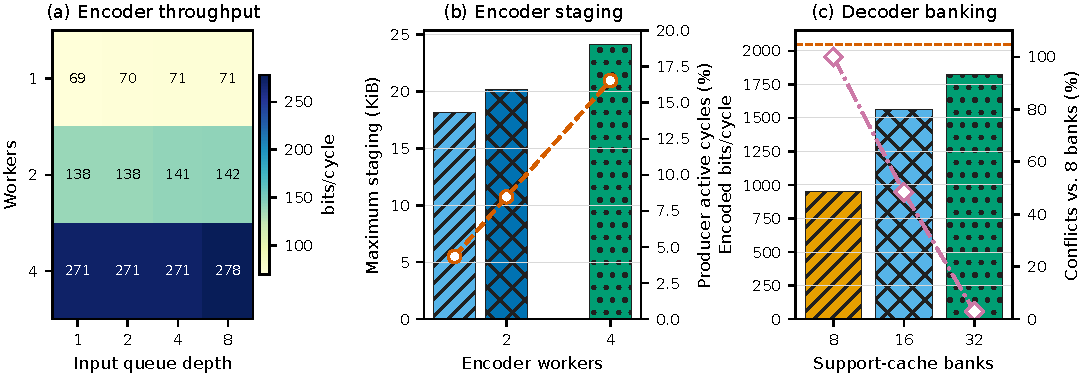
\includegraphics[width=\textwidth]{supplement/figures/figS4_hardware_sensitivity.pdf}
\caption{Finite producer queues and banked reconstruction. (a) Encoder throughput scales primarily with worker count; increasing outstanding-format capacity has negligible throughput effect. (b) Four workers reach 278.1 input bits/cycle with at most 25~KiB of staging in the evaluated surface. Producer stall fraction is measured against an always-ready source and therefore quantifies offered-load saturation. (c) Increasing support-cache banks from 8 to 32 raises median decoder throughput from 949.6 to 1,822.4 encoded bits/cycle, raises lane utilization from 46.4\% to 89.0\%, and reduces conflicts by 97.1\%. Source: \texttt{A7\_encoder\_queue\_surface.csv} and \texttt{A8\_decoder\_banking.csv}.}
\label{fig:s-hardware}
\end{figure*}

The producer surface spans input depth 1/2/4/8, one/two/four workers, and outstanding capacity 2/4/8/16. Worker parallelism dominates the cycle model: one, two, and four workers reach roughly 69, 138, and 271--278 input bits/cycle. Deeper input queues increase staging but improve four-worker throughput only modestly. On the consumer, bank conflicts rather than lane parsing limit the eight-bank case; 32 banks reduce conflicts from 138,496.5 to 3,992 and sustain 1,822.4 encoded bits/cycle.

\section{Robustness and operating regime}
\begin{figure*}[t]
\centering
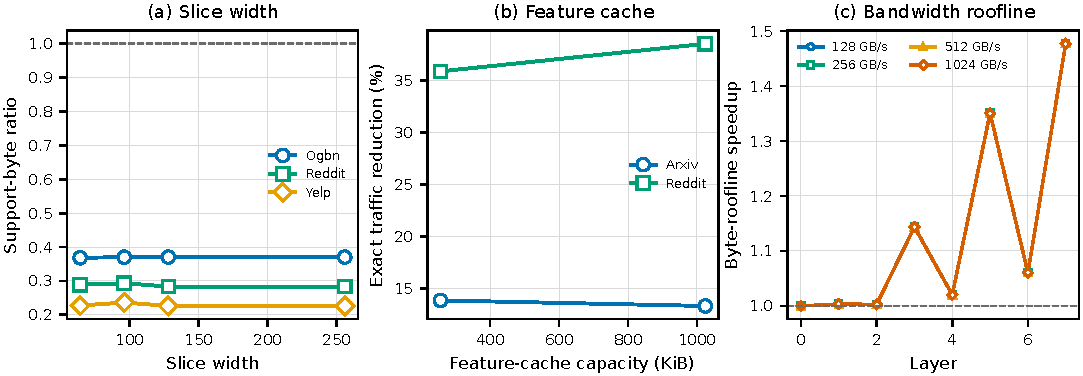
\includegraphics[width=\textwidth]{supplement/figures/figS5_sensitivity.pdf}
\caption{Representation and memory sensitivity. (a) Complete support-byte ratios are stable across 64--256-feature slices for representative primary traces. (b) Increasing feature-cache capacity from 256~KiB to 1~MiB changes exact traffic reduction from 13.85\% to 13.31\% on Arxiv and from 35.87\% to 38.52\% on Reddit. (c) Byte-roofline projections identify layers whose traffic reduction is exposed under memory-bound execution; they identify layers whose traffic reduction is exposed under memory-bound execution. Source: \texttt{A9\_slice\_width.csv}, \texttt{A9\_feature\_cache\_exact\_traffic.csv}, and \texttt{A10\_bandwidth\_roofline\_projection.csv}.}
\label{fig:s-sensitivity}
\end{figure*}

The slice-width result is stable: the complete support representation changes little from width 64 to 256 on the representative Arxiv, Reddit, and Yelp traces, indicating that the gain is not tuned to a single slice width. Cache sensitivity is workload dependent because feature misses can either expose or dilute support traffic. Exact O1 edge ordering retains 13.65\% Arxiv and 33.30\% Reddit traffic reduction. The bandwidth panel is a byte-roofline projection and is used only to explain which layers are memory exposed.

\section{Quality and implementation}
Every primary paired FP8/FP16 quality point lies close to the FP32 result; the maximum absolute difference is 0.053 percentage points. Table~\ref{tab:s-quality} reports all ten compatible primary pairs. The execution model reports 1.220$\times$ for 16-layer Arxiv and 0.994$\times$ for the Chameleon control. CACTI results quantify the bank-count trade-off of the support cache, while routed and synthesized logic results are reported separately below.

\begin{table*}[t]
\centering
\caption{Paired numerical quality for all compatible primary checkpoints. $\Delta$ is FP8/FP16 minus FP32 in percentage points; the arithmetic contract is shared by the baseline and \sys{}.}
\label{tab:s-quality}
\scriptsize
\setlength{\tabcolsep}{5pt}
\begin{tabular}{lrrr@{\hspace{12pt}}lrrr}
\toprule
Trace & FP32 & FP8/FP16 & $\Delta$ (pp) & Trace & FP32 & FP8/FP16 & $\Delta$ (pp) \\
\midrule
Flickr--7  & 0.472460 & 0.472281 & -0.018 & Arxiv--7  & 0.686727 & 0.687036 & +0.031 \\
Flickr--17 & 0.470354 & 0.470174 & -0.018 & Arxiv--17 & 0.682756 & 0.682777 & +0.002 \\
Flickr--27 & 0.472550 & 0.472774 & +0.022 & Arxiv--27 & 0.687118 & 0.686583 & -0.053 \\
Reddit--7  & 0.953557 & 0.953360 & -0.020 & Reddit--17 & 0.947166 & 0.946969 & -0.020 \\
Reddit--27 & 0.947148 & 0.947094 & -0.005 & Yelp--7 & 0.433947 & 0.433952 & +0.001 \\
\bottomrule
\end{tabular}
\end{table*}

\section{Detailed derivations and proofs}
\subsection{Hamming-optimal cohort prototype}
For cohort rows $x_1,\ldots,x_g\in\{0,1\}^C$ and prototype $P\in\{0,1\}^C$, the residual event count is
\begin{align}
E(P)
&=\sum_{r=1}^{g}\lVert x_r\xor P\rVert_0 \\
&=\sum_{r=1}^{g}\sum_{j=1}^{C}\mathbf{1}[x_r[j]\ne P[j]] \\
&=\sum_{j=1}^{C}\sum_{r=1}^{g}\mathbf{1}[x_r[j]\ne P[j]].
\end{align}
Define $n_j=\sum_{r=1}^{g}x_r[j]$. For a fixed column $j$, choosing $P[j]=0$ incurs
\begin{equation}
E_j(0)=\sum_{r=1}^{g}\mathbf{1}[x_r[j]=1]=n_j,
\end{equation}
whereas choosing $P[j]=1$ incurs
\begin{equation}
E_j(1)=\sum_{r=1}^{g}\mathbf{1}[x_r[j]=0]=g-n_j.
\end{equation}
Because columns are independent in the objective,
\begin{align}
\min_{P\in\{0,1\}^C}E(P)
&=\sum_{j=1}^{C}\min_{p\in\{0,1\}}E_j(p) \\
&=\sum_{j=1}^{C}\min(n_j,g-n_j).
\end{align}
Thus an optimizer is
\begin{equation}
P^*[j]=\begin{cases}
1,&n_j>g/2,\\
0,&n_j\le g/2,
\end{cases}
\end{equation}
with zero selected on ties. Since $\min(n_j,g-n_j)\le g/2$ for every $j$,
\begin{equation}
E(P^*)=\sum_{j=1}^{C}\min(n_j,g-n_j)\le\sum_{j=1}^{C}\frac{g}{2}=\frac{gC}{2}.
\end{equation}
The result is nontrivial for hardware because the globally optimal binary prototype is obtained by $C$ independent population counts and comparisons; no iterative or combinatorial search is required.

\subsection{Fixed-partition non-expansion bound}
Let $q$ denote fixed tile boundaries, slice width, headers, and alignment. The anchor selector evaluates a set containing the independent baseline record, hence
\begin{align}
B_A^{\sys}(A_p)
&=\min_{F\in\{\beicsr,\mathrm{A0},\mathrm{A2}\}} B_F^{(q)}(A_p)\\
&\le B_{\beicsr}^{(q)}(A_p).
\end{align}
The target selector compares the delta and independent records, hence
\begin{align}
B_T^{\sys}(A_p,T_p)
&=\min\!\left( B_{\Delta}(A_p\xor T_p),\right.\\
&\hspace{25mm}\left.B_{\beicsr}^{(q)}(T_p)\right)\\
&\le B_{\beicsr}^{(q)}(T_p).
\end{align}
Adding these inequalities gives
\begin{align}
B_{\mathrm{pair}}^{\sys}(A_p,T_p)
&=B_A^{\sys}(A_p)+B_T^{\sys}(A_p,T_p)\\
&\le B_{\beicsr}^{(q)}(A_p)+B_{\beicsr}^{(q)}(T_p).
\end{align}
The inequality holds record by record and therefore also after summing over any trace. It bounds serialized support writes under the common partition $q$; producer/consumer rereads and other traffic components remain explicit in the system evaluation.

\subsection{Exact reconstruction}
For each target pair, $D_p=A_p\xor T_p$. Using associativity, commutativity, and self-inversion of XOR,
\begin{align}
A_p\xor D_p
&=A_p\xor(A_p\xor T_p)\\
&=(A_p\xor A_p)\xor T_p\\
&=0\xor T_p\\
&=T_p.
\end{align}
The equality holds independently for every bit, so reconstruction is exact for the complete support bitmap.

\section{Reproducibility materials}
The accompanying materials include support and physical-byte tables, absolute cycles for all ten eligible checkpoints, scheduler source, recurrence and dependency audits, SCALE-Sim shape data, Ramulator2 outputs, anchor accounting, negative controls, PPA, and CACTI data.

\end{document}
